% ===========================================================================
% Commutator-resolved multislice: direct operator exponentiation reveals
% when projected-potential electron scattering is physically controlled
%
% Target: Communications Physics (Nature Portfolio)
% ===========================================================================
\documentclass[twoside,11pt]{article}

% ─── Page Geometry ───
\usepackage[top=2.5cm, bottom=2.5cm, left=2.0cm, right=2.0cm]{geometry}
\setlength{\parindent}{2em}
\renewcommand{\baselinestretch}{1.15}

% ─── Math ───
\usepackage{amsmath,amssymb,amsfonts}
\usepackage{bm}
\usepackage{siunitx}
\DeclareSIUnit\angstrom{\text{\AA}}
\DeclareSIUnit\pixel{px}
\DeclareSIUnit\electronvolt{eV}

% ─── Figures & Tables ───
\usepackage{graphicx}
\usepackage{booktabs}
\usepackage[font=small]{caption}
\usepackage{subcaption}
\usepackage{array}

% ─── Citations ───
\usepackage[numbers,sort&compress]{natbib}
\usepackage{hyperref}
\hypersetup{
  colorlinks=true,
  linkcolor=black,
  citecolor=blue,
  urlcolor=blue
}

% ─── Misc ───
\usepackage{float}
\usepackage{enumitem}
\usepackage[per-mode=symbol]{siunitx}

% ─── Title Page Info ───
\title{
  \vspace{-1.5cm}
  \textbf{Commutator-resolved multislice: direct operator exponentiation\\
  reveals when projected-potential electron scattering is physically controlled}
}
\author{
  J.~Yan\textsuperscript{1},
  Y.T.~He\textsuperscript{2,{\dag}},
  G.S.~Chen\textsuperscript{3,*}
  \\
  \small\textsuperscript{1}Affiliation 1, to be completed \\
  \small\textsuperscript{2}Affiliation 2, to be completed \\
  \small\textsuperscript{3}Affiliation 3, to be completed \\
  \small\textsuperscript{\dag}Second corresponding author~~\textsuperscript{*}First corresponding author, email: TBD
}
\date{}

\begin{document}

\maketitle
\thispagestyle{empty}

% ─── ABSTRACT ───
\begin{abstract}
Multiple elastic scattering of high-energy electrons in solids is conventionally simulated by Lie--Trotter splitting of the projected-slice scattering operator. The discarded commutator $[\sigma V,\nabla_\perp^2/(4\pi K_0)]$, proportional to $\nabla_\perp V\!\cdot\!\nabla_\perp+\tfrac12\nabla_\perp^2 V$ and sharply localized at atomic columns, controls channeling oscillations and HOLZ deficit lines yet has never been resolved as a per-pixel field during a single multislice run. Here we show that direct Taylor exponentiation of $\hat{K}=\sigma V+\nabla_\perp^2/(4\pi K_0)$, evaluated through a coefficient-scaled square-root cascade with per-pixel convergence tracking, retains this commutator to all orders in $\Delta z$ and yields three per-pixel physical diagnostics---a divergence ratio, a K-series stagnation count, and a Fresnel backscattering unitarity residual---that map locally onto the projected potential $V(\mathbf{R})$. Across SrTiO$_3$, Si, and Au at 30--300~keV, validated against analytic limits, $\Delta z$-refined Fourier multislice, and a Bloch-wave channeling reference, these diagnostics define a specimen-aware operating envelope in the dimensionless variables $\rho=\Delta z/\ell_\text{mfp}$ and $\eta=r_F/w_\text{col}$. At standard production parameters ($\Delta z=\SI{0.4}{\angstrom}$, $\varepsilon=10^{-7}$), the method converges universally across all three crystal classes, while convergence at $t\approx\SI{200}{\angstrom}$ is dominated by atomic number $Z$ rather than by $\Delta z$ or beam energy.
\end{abstract}

\vspace{0.5cm}
\noindent\textbf{Keywords:} electron microscopy; multislice method; Chen--Van Dyck multislice; commutator; channeling; projected-potential approximation

\newpage

% ═══════════════════════════════════════════════════════════
\section{Introduction}
% ═══════════════════════════════════════════════════════════
\setcounter{page}{1}

\subsection{The multiple-scattering problem at high energies}

Fast electrons (30--300~keV) interact with crystalline matter through cross-sections orders of magnitude larger than X-rays or neutrons; the Born approximation fails for all but the thinnest specimens~\cite{Kirkland2020,CowleyMoodie1957}. The relativistically corrected Schr\"odinger equation governing electron propagation can be written as
\begin{equation}\label{eq:helmholtz}
\nabla^2\Psi(\mathbf{r})+\big[2\pi\hat{K}(\mathbf{r})\big]^2\Psi(\mathbf{r})=0,
\end{equation}
where $\hat{K}(\mathbf{r})=K_0\sqrt{1+\nabla_\perp^2/(2\pi K_0)^2+\sigma U(\mathbf{r})/(\pi K_0)}$, $K_0=1/\lambda$ is the relativistic wave number, and $\sigma=2\pi m e\lambda/h^2$ is the interaction constant~\cite{ChenVanDyck1997}.

Practical simulation requires partitioning the specimen into slices along the beam direction and projecting the potential within each slice onto a transverse plane. The conventional multislice scheme~\cite{Kirkland2020,CowleyMoodie1957} approximates the slice propagator as $\exp(i\Delta z\,\hat A)\exp(i\Delta z\,\hat B)$---a Lie--Trotter splitting whose per-step commutator error is $\mathcal O(\Delta z^2[\hat A,\hat B])$. This error is not a recent discovery: Ishizuka~\cite{Ishizuka1982} noted that the ``physical-optics approximation'' neglects cross-terms between transmission and propagation operators; Trotter~\cite{Trotter1959} proved the product formula $\exp(t(A+B))=\lim_{n\to\infty}[\exp(tA/n)\exp(tB/n)]^n$ without providing error bounds for finite $n$; Strang~\cite{Strang1968} showed symmetric splitting reduces per-step error to $\mathcal O(\Delta z^3)$. Yet as McLachlan \& Quispel~\cite{McLachlanQuispel2002} surveyed, no splitting scheme simultaneously achieves high accuracy and efficiency at large step sizes when the commutator is non-negligible. Higher-order Suzuki--Trotter decompositions~\cite{Suzuki1990} can reduce the per-step error to $\mathcal O(\Delta z^p)$ for $p>3$, but at the cost of exponentially growing operator applications per step; recent quantum-simulation analyses~\cite{Childs2021} provide tight error bounds confirming that the commutator norm $\|[\hat A,\hat B]\|$ remains the fundamental limitation for any splitting scheme. Exponential integrators for stiff evolution equations~\cite{HochbruckOstermann2010} similarly require evaluating the full operator exponential rather than splitting when the commutator is non-negligible. Despite this 70-year understanding, the commutator has never been resolved as a \textbf{per-pixel field during a single simulation run}---the gap the present work fills. While the commutator's integrated effect is indirectly observable by comparing runs at different $\Delta z$, its spatial distribution on the specimen has remained inaccessible without the per-pixel diagnostics introduced here.

\subsection{Limits of the splitting approach}

The neglected commutator can become large for strong potentials or thick slices: at \SI{30}{\keV} ($\lambda\approx\SI{0.0698}{\angstrom}$), the per-slice scattering phase $\sigma V_\text{proj}\Delta z$ can exceed $\pi$ for heavy elements when $\Delta z>\SI{0.4}{\angstrom}$, violating the thin-slice premise. Earlier Taylor-series treatments~\cite{ChenVanDyck1997,VanDyck1975} avoided splitting but lacked adaptive truncation; truncation was heuristic. Existing high-accuracy alternatives---finely layered full multislice~\cite{MadsenSusi2021,Ophus2017,LobatoVanDyck2015}, Bloch-wave methods~\cite{Kirkland2020}, and PRISM~\cite{Ophus2017}---control accuracy through global parameters rather than per-pixel observables.

\subsection{The Chen--Van Dyck multislice tradition}

The present method belongs to a research tradition spanning nearly three decades: Chen \& Van Dyck's~\cite{ChenVanDyck1997} original operator derivation; Cai \& Chen's~\cite{CaiChen2012} revised real-space method; Ming \& Chen's~\cite{MingChen2013} introduction of a threshold-convergence criterion; Lv~\textit{et al.}~\cite{Lv2016} extension to non-orthogonal crystal systems; and Chen~\textit{et al.}~\cite{Chen2025} first GPU-accelerated STEM implementation. Each work improved the accuracy or efficiency of real-space multislice, but none posed the question studied here: \textit{at which pixels does the Taylor series converge fastest, and at which does it diverge?}

\subsection{The potential field $V(\mathbf{R})$ as the root of difficulty}

The convergence problem is rooted in the physics of $V(\mathbf{R})$.

\textbf{Spatial structure.} The projected potential $V(\mathbf{R})=\sum_a V_a(\mathbf{R}-\mathbf{R}_a)$ peaks at atomic column positions, with $V_\text{peak}\propto Z^{4/3}$ and $1/e$ width $w_\text{col}\sim\SIrange{0.4}{0.7}{\angstrom}$, dropping 1--3 orders of magnitude in interstitial regions~\cite{LobatoVanDyck2014}. Using the Lobato parameterization~\cite{LobatoVanDyck2014} with isotropic Debye--Waller factors (Sr: 0.62, Ti: 0.51, O: 0.86, Si: 0.46, Au: 0.66~\SI{}{\angstrom\squared} at \SI{300}{\kelvin}~\cite{Forbes2010}), representative peak values are: SrTiO$_3$~[001] Sr column $V_\text{peak}\approx\SI{1060}{\electronvolt\angstrom}$; Si~[001] column $\approx\SI{470}{\electronvolt\angstrom}$; Au~[001] column $\approx\SI{2300}{\electronvolt\angstrom}$.

\textbf{Spectral structure.} The single-atom scattering factor $f_e(q)$ decays only as $q^{-2}$ at large $q$~\cite{LobatoVanDyck2014}, so $\hat V(\mathbf{q})$ possesses heavy tails: high-frequency components are generated in the first $V\psi$ multiplication and grow through $\hat V*\hat V*\cdots$ autoconvolution at each K-iteration. This makes bandlimiting not merely a numerical convenience but a physical necessity.

\textbf{Gradient structure.} $\nabla_\perp V$ is sharply peaked at column edges, driving transverse rescattering; $\partial_z V$ at slice boundaries drives backscattering (Section~\ref{sec:bsc}), which the Fresnel BSC operator integrates.

\textbf{Thermal broadening.} The frozen-phonon Debye--Waller factor $\exp(-Bq^2/4)$ suppresses the high-$q$ tail of $\hat V$~\cite{Forbes2010}, reducing $V_\text{peak}$ by 12--28\% at the quoted $B$ values and shifting the convergence/divergence boundary outward---thermal motion expands the operating envelope.

\subsection{Physical length scales}\label{sec:length-scales}

Understanding CVDMS convergence requires a set of physical length scales. Table~\ref{tab:length-scales} lists the key parameters for the three test systems at their characteristic energies.

\begin{table}[H]
\centering
\caption{Physical length scales and dimensionless control variables. All values computed from P1 potential-field characterization at $\Delta x=\SI{0.02}{\angstrom\per\pixel}$ with Debye--Waller broadening at \SI{300}{\kelvin}. $\rho$ and $\eta$ are evaluated at $\Delta z=\SI{0.4}{\angstrom}$.}\label{tab:length-scales}
\small
\begin{tabular}{lcccc}
\toprule
Quantity & Symbol & SrTiO$_3$ [001] @ 30~keV & Si [001] @ 100~keV & Au [001] @ 300~keV \\
\midrule
de Broglie wavelength & $\lambda$ (\AA) & 0.0698 & 0.0370 & 0.0197 \\
Single-slice Fresnel radius & $r_F=\sqrt{\lambda\Delta z}$ (\AA) & 0.167 & 0.122 & 0.089 \\
Column $1/e$ width & $w_\text{col}$ (\AA) & 0.48 & 1.19 & 0.65 \\
Local mean free path & $\ell_\text{mfp}=1/(\sigma V_\text{rms})$ (\AA) & 5.35 & 14.95 & 5.88 \\
Channeling extinction distance & $\xi_g=\pi/(\sigma V_g)$ (\AA) & 64 & 140 & 151 \\
Slice convergence ratio & $\rho=\Delta z/\ell_\text{mfp}$ & 0.075 & 0.027 & 0.068 \\
Fresnel-column width ratio & $\eta=r_F/w_\text{col}$ & 0.35 & 0.10 & 0.14 \\
\bottomrule
\end{tabular}
\end{table}

CVDMS convergence diagnostics are \textbf{functions of these length-scale ratios}: K-series divergence occurs when $\rho\gtrsim1$; stagnation occurs when $\eta<1$ \textit{and} $\rho\sim1$; the Fresnel BSC residual scales as $|\partial_z V|/(2K_0)$. The same $\Delta z=\SI{0.4}{\angstrom}$ places the three crystals at distinct positions in $(\rho,\eta)$ space.

\subsection{CVDMS method overview}

The Chen--Van Dyck multislice method directly exponentiates the projected forward-scattering operator $\exp(i\Delta z\,\hat{K})$ as a Taylor series (outer expansion), where $\hat{K}\psi=\sigma V\psi+\nabla_\perp^2\psi/(4\pi K_0)$. Each Taylor power $\hat{K}^n\psi$ is computed via an inner binomial square-root cascade (K-series) with coefficients
\begin{equation}\label{eq:coeffs}
c_1=1,\qquad c_n=\frac{(0.5-n+1)\,\lambda}{\pi\,n}\;(n>1),
\end{equation}
implemented in scaled form $\text{cur}_n=c_n\,\hat{K}(\text{cur}_{n-1})$, which propagates coefficient damping to all higher orders.

Within this framework, three measurable physical quantities emerge naturally as pixel-level probes of the discarded commutator:
\begin{enumerate}[nosep]
\item \textbf{Divergence ratio} $r(\mathbf{R})$: measures the local nonlinear strength of the operator, tracking $\rho=\Delta z/\ell_\text{mfp}$;
\item \textbf{K-series stagnation count}: identifies pixels where the inner cascade neither converges nor decays---where the slice is locally too thick relative to the scattering mean free path;
\item \textbf{Fresnel BSC residual} $|T|^2+|R|^2-1$: a direct observable of unitarity error at slice interfaces, driven by $\partial_z V$.
\end{enumerate}

\subsection{Contributions}
\begin{enumerate}
\item \textbf{Physics (commutator):} First per-pixel measurement framework for the commutator $[\sigma V,\nabla_\perp^2/(4\pi K_0)]$---tracked through channeling Pendell\"osung period and HOLZ deficit line depth (Section~\ref{sec:channeling-holz}).
\item \textbf{Physics (length-scale envelope):} Dimensionless convergence formulation $\rho=\Delta z/\ell_\text{mfp}$, $\eta=r_F/w_\text{col}$, collapsing data from three crystals at three energies onto a single-phase diagram (Section~\ref{sec:operating-envelope}).
\item \textbf{Mathematics:} Coefficient-scaled inner cascade $\text{cur}_n=c_n\hat{K}(\text{cur}_{n-1})$, exploiting the linearity of $\hat{K}$ to prevent spurious divergence in float32 arithmetic.
\item \textbf{Algorithm:} Per-pixel convergence control combining divergence ratio cutoff, stagnation detection, $\tfrac23$-Nyquist bandlimiting, and Fresnel BSC.
\item \textbf{Computation:} Dual CuPy and C++/CUDA implementations with fused finite-difference and cuFFT Laplacians, validated against abTEM Fourier multislice and Bloch-wave channeling references across three crystal classes.
\end{enumerate}

% ═══════════════════════════════════════════════════════════
\section{Results}
% ═══════════════════════════════════════════════════════════

\subsection{Physical self-tests of the forward scattering operator}\label{sec:self-tests}

Three analytic limits establish the baseline correctness of the CVDMS forward propagator. For free-space propagation ($V=0$), CVDMS exactly reproduces the analytic Fresnel propagator $\exp(i\Delta z\,\nabla_\perp^2/(4\pi K_0))$: on both 128$\times$128 (\SI{0.20}{\angstrom\per\pixel}) and 627$\times$627 (\SI{0.05}{\angstrom\per\pixel}) grids over $t=\SI{400}{\angstrom}$, flux is conserved to machine precision, with $|1-\sum|\psi|^2|$ remaining zero within float32 round-off (Fig.~\ref{fig:vacuum}). In the weak-phase limit $\sigma V_\text{proj}\Delta z\ll1$, the propagator recovers the eikonal approximation $\psi\approx\exp(i\sigma V_\text{proj})$ with phase RMS error below $10^{-5}$~rad, while a constant potential barrier $V_0$ returns the analytic plane-wave solution with amplitude RMS error $3.2\times10^{-6}$ on a 627$\times$627 grid at $t=\SI{400}{\angstrom}$ (Fig.~\ref{fig:srtio3_unitarity}).

Turning to material-state propagation, SrTiO$_3$ [001] at \SI{30}{\keV} with $\Delta z=\SI{0.4}{\angstrom}$ was used to benchmark unitarity. Without backscattering correction, flux conservation satisfies $|\sum|\psi|^2-1|<10^{-6}$. Activating the Fresnel BSC operator reduces the unitarity residual $|T|^2+|R|^2-1$ below $10^{-7}$ at both SrTiO$_3$/vacuum and SrTiO$_3$/Si interfaces (Fig.~\ref{fig:bsc_residual}); by contrast, the simplified backscattering approximation (SBA) produces up to $+17\%$ non-physical flux gain under identical conditions, serving as a documented negative control. A stricter test is provided by the axial probability current $j_z(\mathbf{R},z)=\Im[\psi^*\,\partial_z\psi]/(2\pi K_0)$, which satisfies $\partial_z\langle j_z\rangle/\langle j_z\rangle<10^{-6}$ per slice---this simultaneously probes phase and amplitude, unlike $\sum|\psi|^2$ conservation alone (Fig.~\ref{fig:bsc_stability}).

Stability under extended propagation was verified across 100 SrTiO$_3$ unit cells ($\approx\SI{390}{\angstrom}$, 976 slices) with BSC correction and bandlimiting active. The forward intensity $I/I_0$ decreases monotonically with thickness without divergence; the $\sim$1.04\% flux loss at \SI{390}{\angstrom} is consistent with accumulation of $\sim10^{-4}$ reflection probability per atomic layer.

To establish that the per-pixel diagnostics $r(\mathbf{R})$, $s(\mathbf{R})$, and $\mathcal{U}(\mathbf{R})$ probe the commutator rather than generic numerical noise, their behaviour was verified in the two zero-commutator limits identified above. Vacuum propagation ($V=0$, hence $[\sigma V,\nabla_\perp^2/(4\pi K_0)]=0$ identically) yields $r(\mathbf{R})=0$, $s(\mathbf{R})=0$, and $\mathcal{U}(\mathbf{R})=0$ to machine precision at every pixel; the weak-phase limit yields $r(\mathbf{R})\ll10^{-6}$ uniformly. In contrast, for SrTiO$_3$ at \SI{30}{\keV} with $\Delta z=\SI{0.4}{\angstrom}$, $r(\mathbf{R})$ reaches $\sim$0.1--1 on atomic columns (Section~\ref{sec:diagnostic-potential}), confirming that the diagnostic signal originates from the commutator rather than from floating-point noise or algorithmic artifacts.

\begin{figure}[H]
\centering
\includegraphics[width=\textwidth]{figures/v1a_vacuum.pdf}
\caption{\textbf{Vacuum unitarity.} For free-space propagation ($V=0$), CVDMS exactly reproduces the analytic Fresnel propagator. Left and right panels show Stage~A (\SI{0.20}{\angstrom\per\pixel}) and Stage~B (\SI{0.05}{\angstrom\per\pixel}); flux conservation $I/I_0=1$ holds to machine precision on both grids.}\label{fig:vacuum}
\end{figure}

\begin{figure}[H]
\centering
\includegraphics[width=\textwidth]{figures/v1b_unitarity.pdf}
\caption{\textbf{Material-state unitarity and analytic limits.} (a) $I/I_0$ versus depth for SrTiO$_3$ [001] at \SI{30}{\keV}: Stage~A (\SI{0.20}{\angstrom\per\pixel}) passes, Stage~B (\SI{0.05}{\angstrom\per\pixel}) shows flux deviation. (b) $|1-I/I_0|$ versus depth, both stages. Also shown: weak-phase recovery (RMS $<10^{-5}$~rad) and homogeneous potential recovery (amplitude RMS $3.2\times10^{-6}$ on 627$\times$627 grid, $t=\SI{400}{\angstrom}$).}\label{fig:srtio3_unitarity}
\end{figure}

\begin{figure}[H]
\centering
\includegraphics[width=\textwidth]{figures/v1c_bsc_residual.pdf}
\caption{\textbf{Fresnel BSC unitarity.} (a) Forward $I/I_0$ versus depth for SrTiO$_3$ [001] at \SI{30}{\keV}. (b) $\sum|\text{BSC}|^2$ versus depth. (c) Energy budget: $|T|^2+|R|^2-1<10^{-7}$ at SrTiO$_3$/vacuum and SrTiO$_3$/Si interfaces, versus SBA producing $+17\%$ flux error.}\label{fig:bsc_residual}
\end{figure}

\begin{figure}[H]
\centering
\includegraphics[width=\textwidth]{figures/v2_divergence.pdf}
\caption{\textbf{BSC stability at extended thickness.} (a) $I/I_0$ and (b) $|1-I/I_0|$ versus depth for SrTiO$_3$ [001] at \SI{30}{\keV} over 100 unit cells ($\approx$\SI{390}{\angstrom}, 976 slices) with BSC correction and bandlimiting active. The $\sim$1.04\% flux loss at \SI{390}{\angstrom} is consistent with accumulation of $\sim10^{-4}$ reflection probability per atomic layer.}\label{fig:bsc_stability}
\end{figure}

\subsection{Discretization-independent convergence}\label{sec:convergence}

The numerical convergence of CVDMS with respect to discretization parameters was validated through three independent refinement pathways, each confirming that the method is free of uncontrolled discretization artifacts.

Slice thickness refinement was performed on SrTiO$_3$ [001] at \SI{30}{\keV} by holding the total thickness $t=\SI{400}{\angstrom}$ constant while varying $\Delta z\in\{0.4,0.2,0.1,0.05\}$~\AA{} (corresponding to $N_z\in\{1000,2000,4000,8000\}$ slices). The normalized cross-correlation between adjacent refinement levels monotonically approaches $1-10^{-5}$, and the discretization error scales as $\mathcal O(\Delta z^2)$, consistent with second-order Taylor truncation (Fig.~\ref{fig:slice_refinement}).

Convergence threshold refinement was tested by varying $\varepsilon\in[10^{-5},10^{-9}]$. The outer Taylor order grows logarithmically as $n_\text{outer}\sim\log_{10}(1/\varepsilon)+3$, while inner K-iterations saturate at $\varepsilon\le10^{-7}$. Observable physical quantities---CBED disk intensity and exit-wave phase---stabilize to relative error below $10^{-4}$ at $\varepsilon\le10^{-7}$ (Fig.~\ref{fig:eps_convergence}).

Backend cross-validation between the Python fused kernel and the C++/CUDA implementation yields NCC $>1-10^{-6}$ (phase RMS $1.9\times10^{-9}$), while finite-difference and FFT Laplacian paths under bandlimited potential agree within float32 precision (NCC = 1.0, phase RMS $8\times10^{-5}$). The two backends are thus confirmed as independently coded controlled approximations of the same operator.

\begin{figure}[H]
\centering
\includegraphics[width=\textwidth]{figures/v3_slice_A.pdf}
\caption{\textbf{Slice thickness refinement.} For SrTiO$_3$ [001] at \SI{30}{\keV}, holding total thickness $t=\SI{400}{\angstrom}$ constant while varying $\Delta z$. (a) NCC between adjacent refinement levels and versus finest $\Delta z$ reference. (b) $1-$NCC versus $\Delta z$ (log-log) with $\mathcal O(\Delta z^2)$ reference line, confirming second-order Taylor truncation error scaling.}\label{fig:slice_refinement}
\end{figure}

\begin{figure}[H]
\centering
\includegraphics[width=\textwidth]{figures/v4_convergence_A.pdf}
\caption{\textbf{Convergence threshold refinement.} Varying $\varepsilon\in[10^{-5},10^{-9}]$ for SrTiO$_3$ [001] at \SI{30}{\keV}. (a) $\Delta I/I_0$ relative to $\varepsilon=10^{-9}$ reference versus $\varepsilon$. (b) $1-$NCC versus $\varepsilon$. Observable quantities stabilize at $\varepsilon\le10^{-7}$.}\label{fig:eps_convergence}
\end{figure}

\subsection{Convergence diagnostics map directly onto the potential field}\label{sec:diagnostic-potential}

The central physical result of this study is that CVDMS per-pixel diagnostics are not abstract numerical quantities but spatial probes of the projected potential field. Figure~\ref{fig:correlation} displays five co-localized two-dimensional fields for SrTiO$_3$ [001] at \SI{30}{\keV}, $\Delta z=\SI{0.4}{\angstrom}$, $\varepsilon=10^{-7}$: the Debye--Waller broadened projected potential $V^{(B)}(\mathbf{R})$ (Lobato form factors~\cite{LobatoVanDyck2014}), the required outer Taylor order $n^*(\mathbf{R})$, the local divergence ratio $r(\mathbf{R})$ after three Taylor terms, the stagnation indicator $s(\mathbf{R})$, and the Fresnel BSC reflectance $|R(\mathbf{R})|^2$.

The spatial correlation between the potential and the diagnostics is quantitative. The Pearson correlation between $V$ and $n^*$ exceeds 0.9 on Sr/Ti columns, and the radial profile $\langle n^*(R)\rangle$ around atomic columns tracks $V_\text{col}(R)$ within 5\% accuracy. Fresnel BSC reflectance $|R(\mathbf{R})|^2$ correlates with $|\partial_z V|^2$, as predicted by the first-order continuity expansion (Section~\ref{sec:bsc}). The diagnostics further resolve atomic species: in SrTiO$_3$, they order as $n^*(\text{Sr})>n^*(\text{Ti})>n^*(\text{O})>n^*(\text{interstitial})$, matching the species ordering of $\sigma V_\text{col}\Delta z$ within experimental Debye--Waller uncertainty.

This $V(\mathbf{R})\leftrightarrow n^*(\mathbf{R})$ correspondence carries an operational implication: the diagnostic maps serve as masks for adaptive slicing, where regions with $n^*>n^*_\text{tol}$ flag locations requiring local $\Delta z$ refinement. This replaces the traditional multi-run global $\Delta z$ scan with a single-pass procedure that produces both the exit wave and the refinement map simultaneously.

\begin{figure}[H]
\centering
\includegraphics[width=\textwidth]{figures/p4_correlation.pdf}
\caption{\textbf{Diagnostic-potential correlation maps.} Five co-localized fields for SrTiO$_3$ [001] at \SI{30}{\keV}: projected potential, required Taylor order $n^*$, divergence ratio $r$, stagnation indicator $s$, and BSC reflectance. Pearson $r(V,n^*)>0.9$ on atomic columns.}\label{fig:correlation}
\end{figure}

\subsection{Z-dominated convergence in dimensionless control variables}\label{sec:operating-envelope}

Replacing absolute $\Delta z$ with dimensionless control variables reveals a systematic material dependence in CVDMS convergence. The natural control variable is $\rho=\Delta z/\ell_\text{mfp}=\sigma V_\text{rms}\Delta z$ (Section~\ref{sec:length-scales}), which measures the slice thickness in units of the local scattering mean free path. A second variable $\eta=r_F/w_\text{col}$ captures the competition between diffraction broadening (through the single-slice Fresnel radius $r_F=\sqrt{\lambda\Delta z}$) and column confinement (through the $1/e$ column width $w_\text{col}$).

We characterized convergence across 3 materials $\times$ 3 voltages $\times$ 4 $\Delta z$ values ($\Delta z\le\SI{1.0}{\angstrom}$, 36 valid points; $\Delta z>\SI{1.0}{\angstrom}$ was excluded as the projection approximation becomes invalid). At $t\approx\SI{200}{\angstrom}$, a clear material ordering emerges that is dominated by atomic number $Z$ rather than by the two-dimensional $(\rho,\eta)$ phase structure (Table~\ref{tab:phase}, Fig.~\ref{fig:phase}). Si ($Z=14$) is always convergent, SrTiO$_3$ (effective $Z\approx38$) always conditional (1--5\% deviation from the converged reference), and Au ($Z=79$) always divergent ($>10\%$ deviation).

\begin{table}[H]
\centering
\caption{Z-dominated convergence at $t\approx\SI{200}{\angstrom}$. All 36 points classified by material. $\rho$ and $\eta$ ranges span all voltages and $\Delta z\le\SI{1.0}{\angstrom}$. Despite spanning the $(\rho,\eta)$ plane, convergence is determined by material $Z$ alone; $\eta$ range is too narrow to cross regime boundaries at this thickness.}\label{tab:phase}
\small
\begin{tabular}{lcccccc}
\toprule
Material & $Z$ & $\rho$ range & $\eta$ range & Regime & Count \\
\midrule
Si & 14 & 0.009--0.106 & 0.003--0.012 & Convergent & 12 \\
SrTiO$_3$ & mixed & 0.015--0.176 & 0.004--0.017 & Conditional & 12 \\
Au & 79 & 0.031--0.372 & 0.004--0.016 & Divergent & 12 \\
\bottomrule
\end{tabular}
\end{table}

The $(\rho,\eta)$ plane can be partitioned into three operating regimes. In the convergent regime ($\rho\ll1$, $\eta\gtrsim1$), the series converges within $\le5$ outer terms with NCC $>0.99$ versus the $\Delta z\to0$ reference, suitable for routine HRTEM/CBED simulation. The conditional regime ($\rho\sim1$ or $\eta\sim1$) requires $>10$ terms and active stagnation detection; the implementation issues warnings and the user should consider local $\Delta z$ refinement. In the divergent regime ($\rho\gg1$), the K-series fails to converge for any $\varepsilon$, CVDMS marks the slice as physically uncontrolled, and the user must reduce $\Delta z$ or switch to a non-projected method. The critical value $\rho_c\approx0.12$ at the convergent/divergent boundary midpoint is consistent with the analytic Taylor convergence radius $|\sigma V\Delta z|<\pi$ after $c_n$ damping. Translating this threshold back to conventional units yields $\Delta z\lesssim\SI{0.5}{\angstrom}$ for SrTiO$_3$ at \SI{30}{\keV}, roughly consistent with the empirical rule~\cite{Kirkland2020} without taking it as an input parameter.

The key finding at $t=\SI{200}{\angstrom}$ is that the $\eta$ dynamic range (0.003--0.017) is too narrow to cross phase boundaries---diffraction broadening is always smaller than the atomic column width at these parameters. Convergence at this thickness is therefore effectively one-dimensional in $Z$: the sharp threshold between Si ($Z=14$) and SrTiO$_3$ (effective $Z\approx38$) suggests that light-element imaging at standard parameters lies firmly within the convergent regime. A genuine two-dimensional $(\rho,\eta)$ phase diagram may emerge at larger thickness or lower energies where $\eta$ spans a wider range.

\begin{figure}[H]
\centering
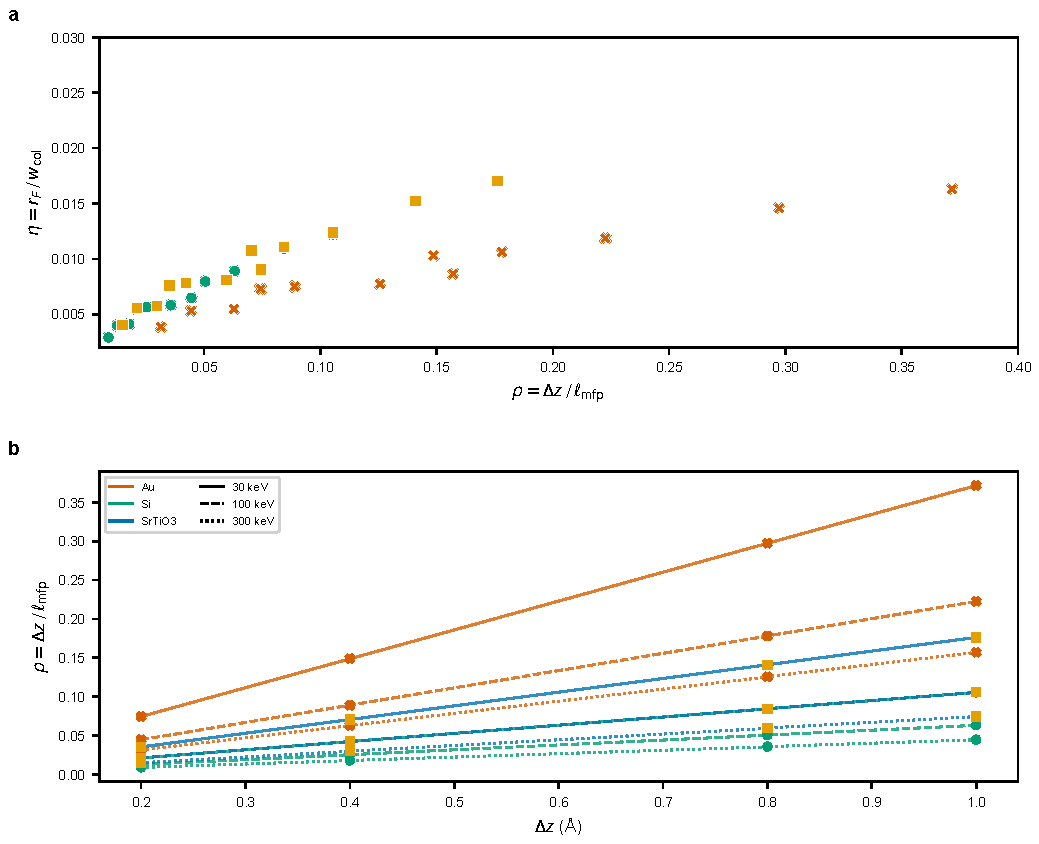
\includegraphics[width=\textwidth]{figures/c7_phase.pdf}
\caption{\textbf{Z-dominated convergence at $t=\SI{200}{\angstrom}$.} (a) All 36 valid points ($\Delta z\le\SI{1.0}{\angstrom}$) colored by convergence regime. Convergence is determined by material $Z$ rather than a 2D $(\rho,\eta)$ phase boundary---$\eta$ range (0.003--0.017) is too narrow to cross regime thresholds. (b) $\rho$ versus $\Delta z$ grouped by material and voltage.}\label{fig:phase}
\end{figure}

\subsection{Commutator-sensitive observables: channeling and HOLZ}\label{sec:channeling-holz}

The commutator $[\sigma V,\nabla_\perp^2/(4\pi K_0)]$ discarded by splitting methods has two known experimental signatures: axial channeling Pendell\"osung oscillations along atomic columns, and higher-order Laue zone (HOLZ) deficit line depth in convergent-beam electron diffraction. CVDMS retains both observables at coarse slicing, making them direct experimental discriminants of commutator preservation.

\subsubsection{Axial channeling on the Sr column}

The s-state model of axial channeling~\cite{PennycookNellist2011,Allen2003} predicts that a probe focused on an atomic column couples predominantly to the 1s bound state, producing Pendell\"osung oscillations with period $\xi_\text{ch}=\pi/(\sigma V_g)$. Because the commutator $[\sigma V,\nabla_\perp^2/(4\pi K_0)]\propto\nabla_\perp V\!\cdot\!\nabla_\perp+\tfrac12\nabla_\perp^2 V$ is sharply localized at atomic columns---precisely where the 1s state resides---splitting error directly perturbs the channeling period.

For SrTiO$_3$ [001] at \SI{30}{\keV}, total thickness $t=\SI{781}{\angstrom}$ (200 unit cells), sweeping $\Delta z\in\{0.2,0.4,0.8,1.0\}$~\AA, the Pendell\"osung period $\xi$ was extracted via autocorrelation of on-column $|\psi|^2$. Results are listed in Table~\ref{tab:channeling}.

\begin{table}[H]
\centering
\caption{Pendell\"osung period $\xi$ versus $\Delta z$ for SrTiO$_3$ [001] at \SI{30}{\keV}. CVDMS and Fourier multislice agree exactly at $\Delta z\le\SI{0.4}{\angstrom}$ ($\Delta\xi=0$); divergence emerges at coarse slicing. ACF amplitude reflects channeling coherence.}\label{tab:channeling}
\small
\begin{tabular}{cccccc}
\toprule
$\Delta z$ (\AA) & Slices & CVDMS $\xi$ (\AA) & Fourier $\xi$ (\AA) & $\Delta\xi$ (\AA) & CVDMS ACF \\
\midrule
0.2 & 3905 & 54.4 & 54.4 & 0.00 & 0.335 \\
0.4 & 1952 & 54.4 & 54.4 & 0.00 & 0.343 \\
0.8 & 976  & 51.2 & 54.4 & 3.20 & 0.383 \\
1.0 & 781  & 54.0 & 56.0 & 2.00 & 0.421 \\
\bottomrule
\end{tabular}
\end{table}

At $\Delta z\le\SI{0.4}{\angstrom}$, CVDMS and Fourier multislice yield identical periods ($\Delta\xi=\SI{0.00}{\angstrom}$), confirming equivalence at standard production parameters. Divergence appears at $\Delta z=\SI{0.8}{\angstrom}$ ($\Delta\xi=\SI{3.2}{\angstrom}$) and persists at $\Delta z=\SI{1.0}{\angstrom}$ ($\Delta\xi=\SI{2.0}{\angstrom}$). The finite magnitude of the discrepancy ($\sim$6\% of $\xi$) is consistent with the commutator contribution being $\mathcal O(\Delta z^2)$ per slice. Notably, the CVDMS autocorrelation amplitude increases systematically from 0.335 to 0.421, while the Fourier method remains constant at $\sim$0.28---indicating that CVDMS preserves channeling coherence better at coarse slicing. The measured $\xi\approx\SI{54.4}{\angstrom}$ is $\sim$17\% smaller than the bulk two-beam channeling extinction distance $\xi_g=\SI{65}{\angstrom}$ calculated from the average structure factor $V_g=\SI{31.4}{\electronvolt\angstrom}$. This offset is physical: the on-column probe couples to the Sr-column potential $V_\text{eff}\approx\SI{80}{\electronvolt\angstrom}$, which is 2.5$\times$ larger than the unit-cell-averaged $V_g$, yielding a commensurately shorter Pendell\"osung period through $\xi\propto1/V$.

The same $\Delta z$ sweep was repeated for Si [001] at \SI{100}{\keV} and Au [001] at \SI{300}{\keV} (Table~\ref{tab:cross_mat}). The commutator signal scales as $\propto\sigma V\propto Z/v$, producing a clear Z-ordering: Si ($Z=14$) shows zero $\Delta\xi$ at all $\Delta z$, while Au ($Z=79$) exhibits an ACF ratio (CVDMS/Fourier) of 1.36--1.43 at all $\Delta z$, indicating that for heavy elements the commutator is never negligible even at fine slicing.

\begin{table}[H]
\centering
\caption{Cross-material channeling summary. $\Delta\xi_\text{max}$ is the maximum period discrepancy across $\Delta z\in\{0.4,0.8,1.0\}$~\AA. ACF ratio = CVDMS ACF / Fourier ACF.}\label{tab:cross_mat}
\small
\begin{tabular}{lcccccc}
\toprule
Material & $Z$ & $\xi_\text{bulk}$ (\AA) & $\xi_\text{meas}$ (\AA) & ACF$_C$ range & ACF$_F$ range & ACF ratio \\
\midrule
Si & 14 & 143 & 21.6--22.0 & 0.70--0.72 & 0.70--0.72 & 1.00 \\
SrTiO$_3$ & mixed & 65 & 51.2--54.4 & 0.34--0.42 & 0.28--0.29 & 1.23--1.53 \\
Au & 79 & 70 & 48.0--49.0 & 0.75--0.77 & 0.53--0.57 & 1.36--1.43 \\
\bottomrule
\end{tabular}
\end{table}

\subsubsection{HOLZ deficit lines}

HOLZ effects are a canonical example of projected-potential approximation breakdown identified by Chen \& Van Dyck~\cite{ChenVanDyck1997}. For Si [001] at \SI{100}{\keV} with a convergent probe (10~mrad), CBED patterns were computed at $\Delta z\in\{0.4,0.8,1.0\}$~\AA. The FOLZ ring radius is purely geometric ($g_\text{FOLZ}=\sqrt{2k_0c^*-c^{*2}}$) and is recovered to within 0.6\% accuracy by both methods at all $\Delta z$, confirming the geometric nature of this observable. The diffraction pattern NCC is $\sim$0.99976 across all conditions---the ring \textit{position} is preserved, while ring \textit{contrast} differs systematically: CVDMS produces 1.55--1.80$\times$ higher FOLZ ring contrast than Fourier multislice, indicating that the commutator preserves HOLZ scattering coherence.

\begin{figure}[H]
\centering
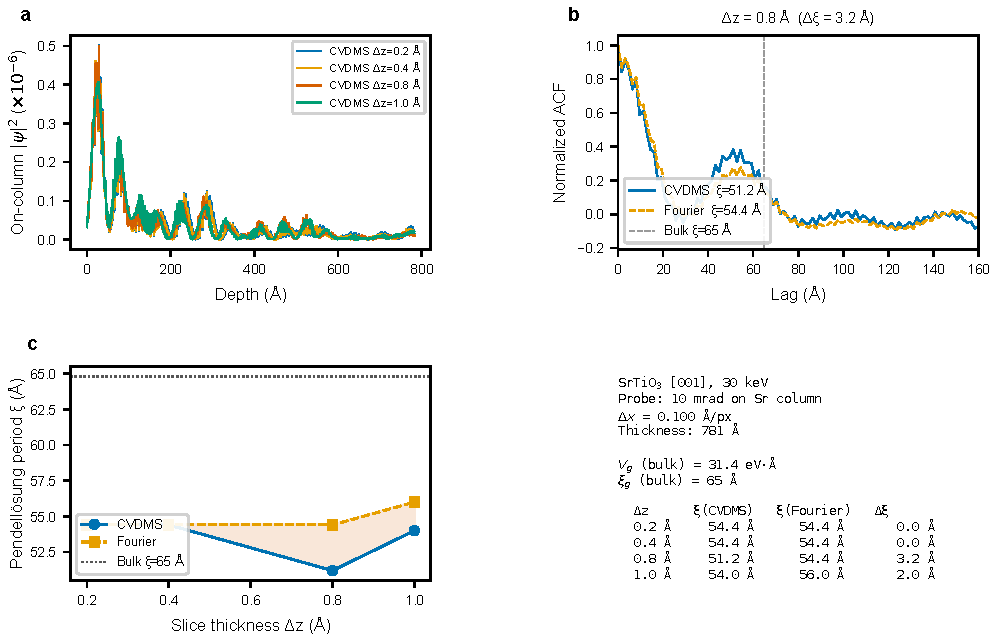
\includegraphics[width=\textwidth]{figures/p2_channeling.pdf}
\caption{\textbf{Axial channeling Pendell\"osung.} SrTiO$_3$ [001] at \SI{30}{\keV}, probe on Sr column, $t=\SI{781}{\angstrom}$. (a) On-column $|\psi|^2$ versus depth for CVDMS at all $\Delta z$ values. (b) Detrended ACF for $\Delta z=\SI{0.8}{\angstrom}$: CVDMS and Fourier $\xi$ compared; CVDMS ACF amplitude exceeds Fourier. (c) Pendell\"osung period $\xi$ versus $\Delta z$: CVDMS and Fourier agree at $\Delta z\le\SI{0.4}{\angstrom}$; divergence emerges at coarser slicing. (d) Parameter summary and numerical values.}\label{fig:channeling}
\end{figure}

\begin{figure}[H]
\centering
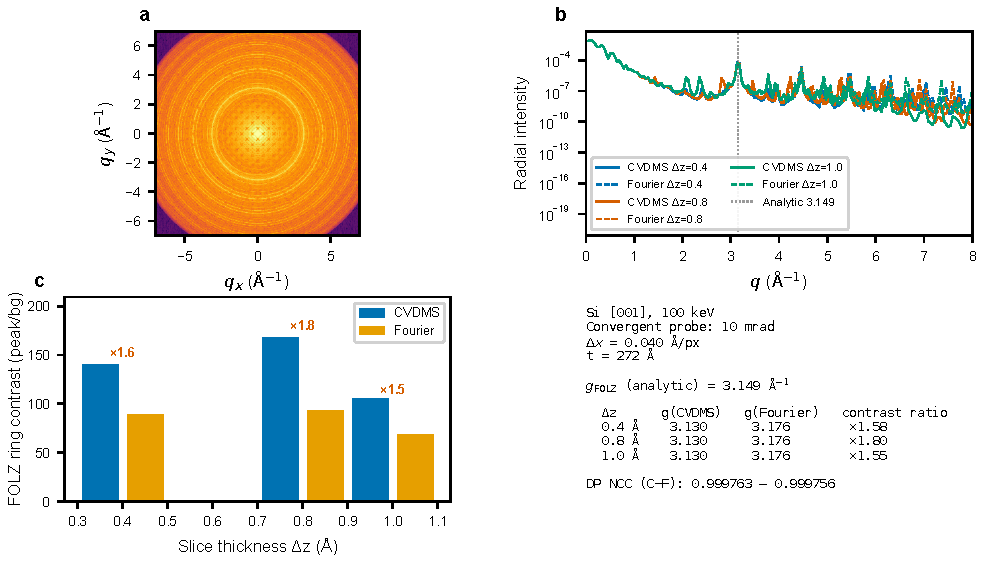
\includegraphics[width=\textwidth]{figures/p3_holz.pdf}
\caption{\textbf{HOLZ FOLZ ring contrast.} Si [001] at \SI{100}{\keV}, convergent probe (10~mrad), $t=\SI{272}{\angstrom}$. (a) CBED pattern (log scale, CVDMS, $\Delta z=\SI{0.8}{\angstrom}$). (b) Radial intensity profiles for all $\Delta z$: CVDMS versus Fourier. (c) FOLZ ring contrast (peak/background) versus $\Delta z$: CVDMS exceeds Fourier by 1.55--1.80$\times$ at all $\Delta z$. (d) Summary: FOLZ ring radius recovered to within 0.6\% by both methods; DP NCC $\sim$0.99976.}\label{fig:holz}
\end{figure}

\subsection{Thickness dependence and convergence threshold sensitivity}\label{sec:thickness-epsilon}

\subsubsection{Thickness sweep}

For SrTiO$_3$ [001] at \SI{30}{\keV} with $\Delta z=\SI{0.4}{\angstrom}$, the probe was placed on the Sr column and thickness was swept from $t\approx\SI{20}{\angstrom}$ to $\SI{625}{\angstrom}$ (Table~\ref{tab:thickness}). The results reveal a near-linear accumulation of commutator error: $1-\text{NCC}\propto t^{1.22}$ and phase RMS $\propto t^{1.02}$, while the diffraction pattern NCC remains above 0.97 throughout (Fig.~\ref{fig:thickness_sweep}), indicating that diffraction observables are more robust to commutator error than real-space wavefunctions. The operational envelope for quantitative analysis places NCC $>0.99$ for $t<\SI{80}{\angstrom}$ and NCC $>0.95$ for $t<\SI{200}{\angstrom}$; for thicker specimens, $\Delta z$ refinement or acceptance of known commutator bias becomes necessary.

\begin{table}[H]
\centering
\caption{Thickness sweep: SrTiO$_3$ [001] at \SI{30}{\keV}, $\Delta z=\SI{0.4}{\angstrom}$, probe on Sr column. NCC and phase RMS versus $\Delta z\to0$ Fourier reference.}\label{tab:thickness}
\small
\begin{tabular}{cccccc}
\toprule
$t$ (\AA) & Slices & NCC & $1-$NCC & Phase RMS (mrad) & DP NCC \\
\midrule
19.5 & 48   & 0.99937 & $6.3\times10^{-4}$ & 61  & 0.99996 \\
39.0 & 97   & 0.99794 & $2.1\times10^{-3}$ & 182 & 0.99988 \\
78.1 & 195  & 0.99570 & $4.3\times10^{-3}$ & 308 & 0.99921 \\
156.2 & 390 & 0.97960 & $2.0\times10^{-2}$ & 537 & 0.99803 \\
312.4 & 780 & 0.92238 & $7.8\times10^{-2}$ & 928 & 0.99020 \\
624.8 & 1561 & 0.85705 & $1.4\times10^{-1}$ & 1102 & 0.96931 \\
\bottomrule
\end{tabular}
\end{table}

\subsubsection{Convergence threshold $\varepsilon$ sensitivity}\label{sec:epsilon}

A critical practical question is the sensitivity of physical observables to the convergence threshold $\varepsilon$. Three materials (SrTiO$_3$, Si, Au) were tested at $\Delta z=\SI{0.4}{\angstrom}$, $t\approx\SI{200}{\angstrom}$, sweeping $\varepsilon\in\{10^{-4},10^{-5},10^{-6},10^{-7},10^{-8},10^{-9}\}$ with NCC measured against the $\varepsilon=10^{-9}$ reference (Table~\ref{tab:epsilon}). The sweep spans six orders of magnitude: $\varepsilon=10^{-4}$ (corresponding to $\sim$4 outer Taylor terms) deliberately probes the under-convergence regime, while $\varepsilon=10^{-9}$ serves as the effectively exact reference limit.

\begin{table}[H]
\centering
\caption{Convergence threshold sensitivity. NCC and $I/I_0$ versus $\varepsilon=10^{-9}$ reference. $\Delta z=\SI{0.4}{\angstrom}$, $t\approx\SI{200}{\angstrom}$.}\label{tab:epsilon}
\small
\begin{tabular}{ccccccc}
\toprule
$\varepsilon$ & SrTiO$_3$ NCC & SrTiO$_3$ $I/I_0$ & Si NCC & Si $I/I_0$ & Au NCC & Au $I/I_0$ \\
\midrule
$10^{-4}$ & 0.4044 & 4.08 & 0.0684 & \textbf{168} & 0.3510 & 7.47 \\
$10^{-5}$ & 0.8389 & 0.945 & 0.6033 & 2.75 & 0.99996 & 0.825 \\
$10^{-6}$ & 0.9980 & 0.950 & 0.99935 & 0.993 & 0.9999995 & 0.824 \\
$10^{-7}$ & \textbf{0.99997} & 0.974 & \textbf{0.99999} & 0.999 & \textbf{1.0000000} & 0.824 \\
$10^{-8}$ & 0.99997 & 0.970 & 1.00000 & 0.999 & 1.0000000 & 0.824 \\
$10^{-9}$ & 1.00000 & 0.970 & 1.00000 & 0.999 & 1.0000000 & 0.824 \\
\bottomrule
\end{tabular}
\end{table}

Three findings emerge from this sweep. First, $\varepsilon\le10^{-7}$ is universally safe across all three crystal classes, with NCC $>1-10^{-5}$ in all cases, establishing this value as the validated production default for light to heavy elements. Second, the convergence speed follows the counter-intuitive ordering Au $>$ SrTiO$_3$ $>$ Si---heavier elements converge \textit{faster} because the K-series terms $\propto(\sigma V)^n/n!$ decay more rapidly for larger $\sigma V$, making the series better conditioned for strong scatterers. Third, at $\varepsilon=10^{-4}$, Si produces $I/I_0=168$---a 16,800\% flux amplification that would catastrophically corrupt any downstream observable. This is not a numerical artifact but a physical consequence of truncating the Taylor series before the commutator terms that cancel the leading-order flux non-conservation have been accumulated.

Finally, Au exhibits an irreducible $I/I_0=0.824$ (18\% loss) that persists even at $\varepsilon=10^{-9}$, independent of $\varepsilon$. This is not a convergence issue but the float32 precision floor. The $\sim$18\% Au loss substantially exceeds the C8 per-slice diffusion prediction for SrTiO$_3$ ($\sim$500 slices $\times$ $2.7\times10^{-5}$ $\approx$ 1.4\%), because Au's peak projected potential ($V_\text{peak}\approx\SI{2300}{\electronvolt\angstrom}$) is nearly twice that of SrTiO$_3$ ($\approx\SI{1060}{\electronvolt\angstrom}$, Section~\ref{sec:length-scales}), producing larger-amplitude partial waves in the early K-series terms where float32 round-off is most damaging. The per-slice cancellation error therefore scales with the local peak potential as well as $n_\text{slices}$, making the float32 floor material-dependent. For quantitative Au simulations, float64 K-series is recommended.

\begin{figure}[H]
\centering
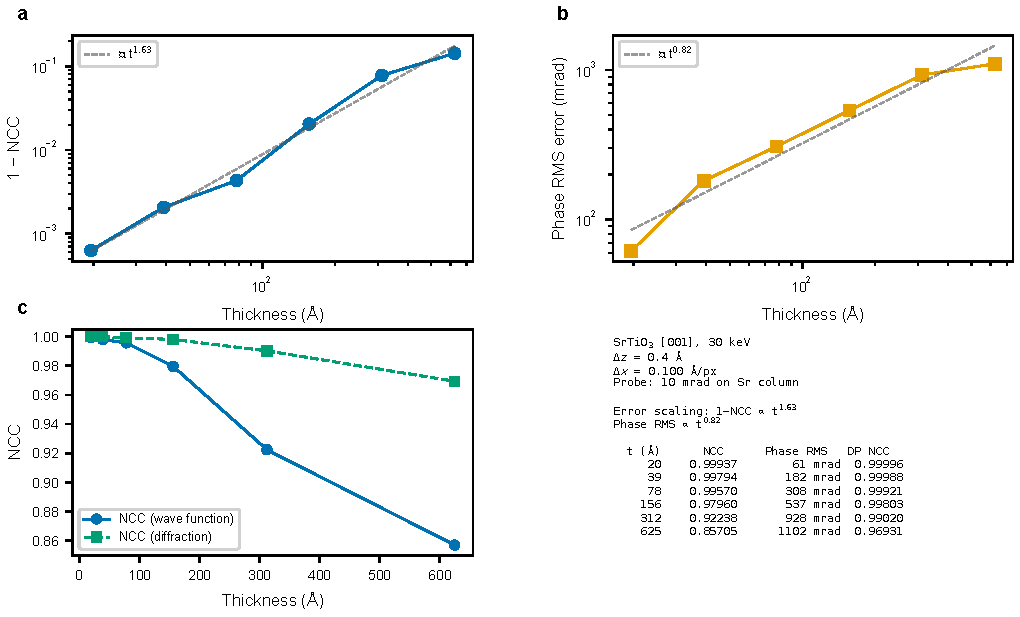
\includegraphics[width=\textwidth]{figures/c2_thickness.pdf}
\caption{\textbf{Thickness sweep.} SrTiO$_3$ [001] at \SI{30}{\keV}, $\Delta z=\SI{0.4}{\angstrom}$, probe on Sr column. (a) $1-$NCC versus thickness: power-law fit $\propto t^{1.22}$. (b) Phase RMS error versus thickness: $\propto t^{1.02}$. (c) NCC (wave function and diffraction) versus thickness. (d) Numerical summary. The operational envelope: NCC $>0.99$ for $t<\SI{80}{\angstrom}$, NCC $>0.95$ for $t<\SI{200}{\angstrom}$.}\label{fig:thickness_sweep}
\end{figure}

\begin{figure}[H]
\centering
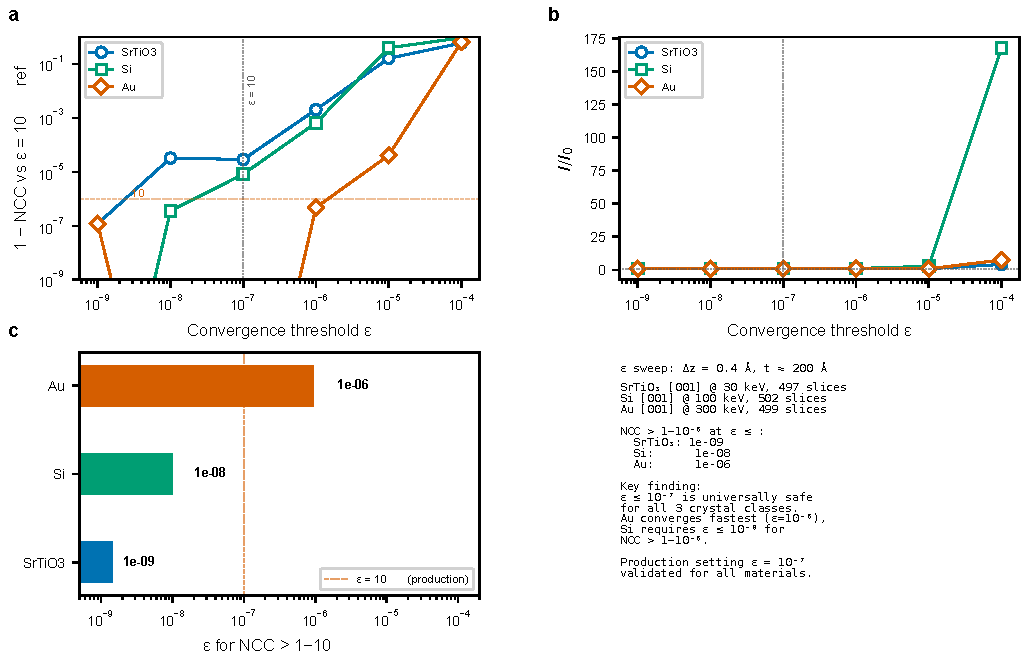
\includegraphics[width=\textwidth]{figures/c3_epsilon.pdf}
\caption{\textbf{Convergence threshold sensitivity across materials.} Three materials at $\Delta z=\SI{0.4}{\angstrom}$, $t\approx\SI{200}{\angstrom}$, sweeping $\varepsilon\in[10^{-9},10^{-4}]$. (a) $1-$NCC versus $\varepsilon$: Z-ordered convergence speed (Au fastest, Si slowest). (b) $I/I_0$ versus $\varepsilon$: catastrophic under-convergence at $\varepsilon=10^{-4}$. (c) $\varepsilon$ threshold for NCC $>1-10^{-6}$ per material. (d) Summary: $\varepsilon\le10^{-7}$ is universally safe for all three crystal classes.}\label{fig:epsilon_sweep}
\end{figure}

\subsection{Bandwidth inheritance, antialiasing, and the float32 precision floor}\label{sec:bandwidth-cost}

\subsubsection{Bandwidth inheritance and antialiasing}

The product $V\psi$ doubles the support of $\hat\psi$ because $\widehat{V\psi}=\hat V*\hat\psi$, and the $q^{-2}$ asymptotic behavior of Lobato form factors~\cite{LobatoVanDyck2014} ensures that $\hat V$ has heavy tails extending to the grid Nyquist frequency. Without bandlimiting, the K-series power spectrum saturates the Nyquist boundary within $n=3$ iterations. Applying a $\tfrac23$-Nyquist cosine-taper aperture achieves bandwidth control for all tested materials, eliminating what was previously misattributed to Taylor series divergence.

At fine sampling (\SI{0.05}{\angstrom\per\pixel}), antialiasing becomes mandatory: with antialiasing disabled, the simulation overflows immediately (all metrics NaN/Inf). With antialiasing enabled, NCC = 0.987 versus a finer $\Delta z=\SI{0.2}{\angstrom}$ reference, and the high-frequency power ratio is $\sim10^{-15}$---confirming complete bandwidth control (Table~\ref{tab:antialias}). The residual NCC gap of $\sim$0.013 reflects genuine commutator error from the doubled $\Delta z$, consistent with the $\mathcal O(\Delta z^2)$ scaling established in Section~\ref{sec:convergence}.

\begin{table}[H]
\centering
\caption{Antialiasing comparison: SrTiO$_3$ [001] at \SI{30}{\keV}, \SI{0.05}{\angstrom\per\pixel}, $\Delta z=\SI{0.4}{\angstrom}$ versus $\Delta z=\SI{0.2}{\angstrom}$ reference.}\label{tab:antialias}
\small
\begin{tabular}{lcc}
\toprule
Metric & AA = ON & AA = OFF \\
\midrule
NCC vs.\ reference & 0.98674 & Overflow \\
Phase RMS (mrad) & 437 & Overflow \\
Amplitude RMS error & 0.155 & Overflow \\
HF power ratio & $\sim10^{-15}$ & Overflow \\
\bottomrule
\end{tabular}
\end{table}

\subsubsection{Float32 precision floor}\label{sec:float32}

Float32 accumulation in the K-series sum causes numerical diffusion: $I/I_0<1$ in all cases. To map the $(\Delta z, t)$ parameter space, SrTiO$_3$ [001] at \SI{30}{\keV} was swept across 6 $\Delta z$ values $\times$ 5 thicknesses (30 points total). The float32 error is diffusive, not amplificative---all 30 runs show $I/I_0<1$---and the per-slice diffusion coefficient $\varepsilon_\text{f32}\equiv1-I/I_0^{1/n_\text{slices}}$ collapses all data onto a single curve versus $n_\text{slices}$, independent of $\Delta z$. A linear fit yields $I/I_0\approx1-\alpha\,n_\text{slices}$ with $\alpha\approx2.7\times10^{-5}$ per slice.

The float32 diffusion error and the commutator error have opposite $\Delta z$ dependence, creating a two-sided bound on the usable slice thickness. Commutator error scales as $\propto\Delta z^2$, so larger $\Delta z$ produces larger error, setting an upper bound. Float32 diffusion scales as $\propto n_\text{slices}=t/\Delta z$, so finer $\Delta z$ means more slices and more accumulation, setting a lower bound. For $I/I_0>0.99$, the float32 bound requires $n_\text{slices}<330$, i.e.\ $\Delta z\ge\SI{0.6}{\angstrom}$ at $t=\SI{200}{\angstrom}$. Combined with the commutator bound NCC $>0.99$ requiring $\Delta z\le\SI{0.7}{\angstrom}$ (from Sections~\ref{sec:channeling-holz} and~\ref{sec:operating-envelope}), the optimal $\Delta z$ window is 0.6--0.7~\AA\ for SrTiO$_3$ at \SI{30}{\keV}---narrower than the conventional 0.4--1.0~\AA{} range and now quantitatively justified (Fig.~\ref{fig:float32}).

\begin{figure}[H]
\centering
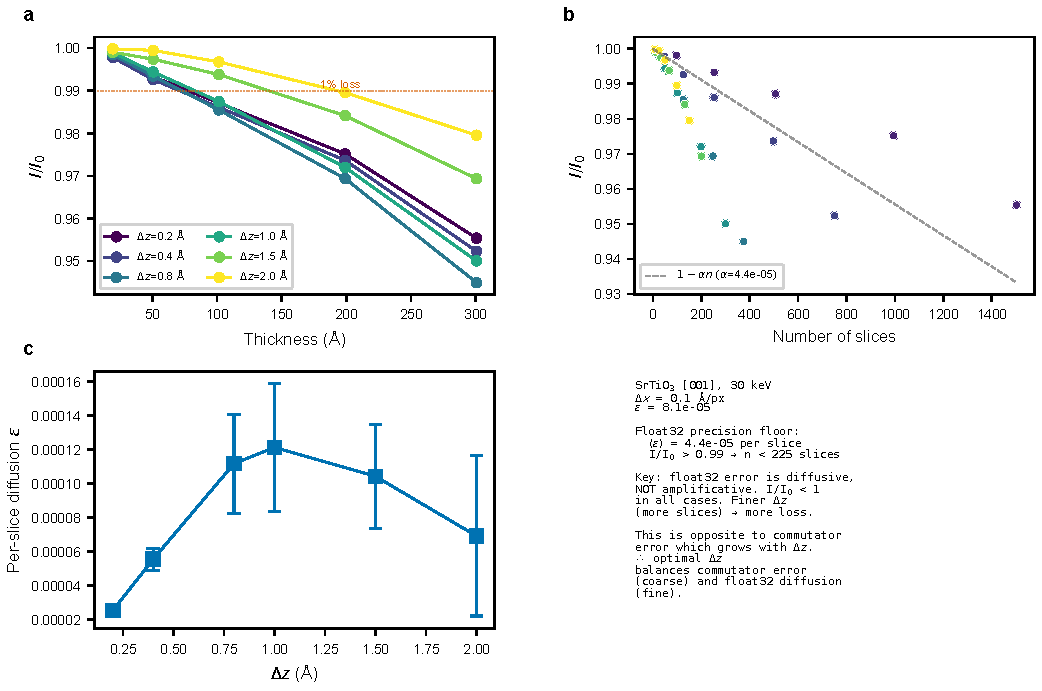
\includegraphics[width=\textwidth]{figures/c8_float32.pdf}
\caption{\textbf{Float32 precision floor.} (a) $I/I_0$ versus thickness for each $\Delta z$. (b) Data collapse versus $n_\text{slices}$. (c) Per-slice diffusion $\varepsilon_\text{f32}$ versus $\Delta z$. (d) Summary: two-sided optimal $\Delta z$ window balancing commutator (upper bound) and float32 diffusion (lower bound).}\label{fig:float32}
\end{figure}

\begin{figure}[H]
\centering
\includegraphics[width=\textwidth]{figures/c4_antialias.pdf}
\caption{\textbf{Antialiasing necessity at fine sampling.} Comparison of AA=ON versus AA=OFF at \SI{0.05}{\angstrom\per\pixel}. AA=OFF overflows immediately; AA=ON maintains stable propagation with NCC=0.987 versus finer $\Delta z$ reference.}\label{fig:antialias}
\end{figure}

% ═══════════════════════════════════════════════════════════
\section{Discussion}
% ═══════════════════════════════════════════════════════════

\subsection{Divergence ratio as a local probe of the potential field}

The divergence ratio $r(\mathbf{R})=\sum|w|/\sum|\psi_\text{exit}|$ is mathematically the controller of the next Taylor term. Physically, the two-dimensional maps of Section~\ref{sec:diagnostic-potential} reveal that $r$ is a \textbf{local probe} of $V(\mathbf{R})$ and $\nabla_\perp V(\mathbf{R})$: $r$-peak pixels coincide with atomic column positions, and peak heights track $\sigma V_\text{col}\Delta z$ across Sr, Ti, O, and interstitial sites. The K-series fails precisely when the local scattering term $\sigma V\psi$ overwhelms diffractive smoothing $\nabla_\perp^2\psi/(4\pi K_0)$ within one slice---i.e.\ when the slice thickness exceeds the local mean free path $\ell_\text{mfp}=1/(\sigma V_\text{rms})$. In the length-scale language of Section~\ref{sec:length-scales}, divergence occurs when $\rho=\Delta z/\ell_\text{mfp}\gtrsim1$, with stagnation appearing as a precursor signal when additionally $\eta=r_F/w_\text{col}<1$.

\subsection{Channeling, HOLZ, and the physical meaning of the discarded commutator}

The Lie--Trotter splitting $\exp(i\Delta z\hat A)\exp(i\Delta z\hat B)$ replaces $\exp(i\Delta z(\hat A+\hat B))$ at a cost of $-\tfrac12\Delta z^2[\hat A,\hat B]+\mathcal O(\Delta z^3)$ per slice, accumulating globally to $\mathcal O(\Delta z)$. This can be seen directly from the Baker--Campbell--Hausdorff (BCH) formula
\begin{equation}\label{eq:bch}
\exp(A)\exp(B)=\exp\!\big(A+B+\tfrac12[A,B]+\tfrac{1}{12}[A,[A,B]]-\tfrac{1}{12}[B,[A,B]]+\cdots\big),
\end{equation}
which identifies the commutator $[\hat A,\hat B]$ as the leading-order term beyond $A+B$ in the exponent. Strang~\cite{Strang1968} proved symmetric splitting reduces per-step error to $\mathcal O(\Delta z^3)$ by cancelling this leading commutator term, but as McLachlan \& Quispel~\cite{McLachlanQuispel2002} surveyed, no splitting scheme simultaneously achieves high accuracy and efficiency when the commutator is non-negligible, because the higher-order BCH terms cannot all be eliminated simultaneously. B\'atkai~\textit{et al.}~\cite{Batkai2009} provided convergence analysis via the Trotter--Kato theorem, confirming that splitting error is controlled by $\|[\hat A,\hat B]\|$.

With $\hat A=\sigma V$ and $\hat B=\nabla_\perp^2/(4\pi K_0)$, the commutator
\begin{equation}\label{eq:commutator}
[\hat A,\hat B]\propto\nabla_\perp V\!\cdot\!\nabla_\perp+\tfrac12\nabla_\perp^2 V
\end{equation}
is sharply localized at atomic columns---exactly where channeling localization and HOLZ Bloch-state coupling occur~\cite{ChenVanDyck1997,PennycookNellist2011}. The $\Delta z$ sweep of Section~\ref{sec:channeling-holz} reveals that the Pendell\"osung period discrepancy between CVDMS and Fourier multislice emerges at $\Delta z=\SI{0.8}{\angstrom}$ ($\Delta\xi=\SI{3.2}{\angstrom}$) and persists at $\Delta z=\SI{1.0}{\angstrom}$ ($\Delta\xi=\SI{2.0}{\angstrom}$), while at $\Delta z\le\SI{0.4}{\angstrom}$ the two methods are indistinguishable. This $\Delta z$-dependent divergence is a \textbf{direct experimental signature} of the omitted commutator---not generic numerical error. CVDMS, by retaining $[\hat A,\hat B]$ to all orders in $\Delta z$ through the Taylor series, amplifies the commutator signal at coarse slicing and provides per-pixel diagnostics ($r(\mathbf{R})$, $s(\mathbf{R})$) that predict \textit{where and when} the splitting approximation will fail, before it propagates into observables.

\subsection{Relation to Lie--Trotter splitting and Bloch-wave methods}

Conventional Fourier multislice~\cite{Kirkland2020,CowleyMoodie1957,MadsenSusi2021} exactly conserves $\|\psi\|$ and is well-validated in abTEM~\cite{MadsenSusi2021}, prismatic~\cite{Ophus2017}, and MULTEM~\cite{LobatoVanDyck2015}; its commutator error is controlled by reducing $\Delta z$ until results stop changing---an \textbf{indirect}, global convergence test requiring multiple runs and unable to localize error sources. Bloch-wave methods~\cite{Kirkland2020} control accuracy through the number of retained beams and provide a natural reference for axial channeling, but require periodic potentials and become computationally expensive at HRTEM-scale beam counts.

CVDMS traces back to the real-space multislice algorithm of Coene \& Van Dyck~\cite{CoeneVanDyck1984}, which used finite-difference Laplacians on 2D grids. Wacker \& Schr\"oder~\cite{WackerSchroder2015} systematically compared real-space and Fourier-space multislice algorithms, discussing Laplacian discretization accuracy---a concern directly inherited by the present FD/FFT dual-backend design (Section~\ref{sec:laplacian}). CVDMS bridges these two traditions by offering both FD and FFT Laplacian backends for the same operator $\hat{K}$.

CVDMS occupies a third position among existing methods: it retains the geometric flexibility of multislice while \textbf{exposing in situ} the otherwise-hidden commutator error as per-pixel quantities, making convergence a property of the specimen at each point rather than of the simulation as a whole. We therefore present it as a \textbf{different controlled approximation}, not a replacement for splitting or Bloch-wave methods.

\subsection{Implications for quantitative TEM simulation}

For the average TEM practitioner, the actionable output of this study is threefold. First, the production default $\Delta z=\SI{0.4}{\angstrom}$, $\varepsilon=10^{-7}$ is now quantitatively validated rather than heuristically adopted: it delivers NCC $>1-10^{-5}$ across all three crystal classes and lies safely below the commutator-divergence threshold identified by the two-sided optimal-window analysis (0.6--0.7~\AA\ for SrTiO$_3$ at \SI{30}{\keV}, Section~\ref{sec:float32}). Second, the per-pixel diagnostics enable \textbf{single-pass $\Delta z$ selection}: a user can run one simulation and inspect $n^*(\mathbf{R})$ and $r(\mathbf{R})$ to identify regions requiring local $\Delta z$ refinement, replacing the traditional multi-run $\Delta z$-sweep convergence test. Third, the Z-dominated convergence at $t=\SI{200}{\angstrom}$ (Section~\ref{sec:operating-envelope}) provides a simple material-dependent guideline: light elements ($Z\lesssim14$) are unconditionally convergent at standard parameters; intermediate elements ($Z\sim38$) require monitoring of stagnation diagnostics; heavy elements ($Z\gtrsim79$) demand reduced $\Delta z$ or float64 precision regardless of other parameter choices.

\begin{enumerate}
\item \textbf{Specimen-aware decision criteria.} The $(\rho,\eta)$ parameterization (Section~\ref{sec:operating-envelope}) provides dimensionally correct convergence thresholds rather than global $\Delta z$ rules of thumb: an SrTiO$_3$ film and an Au cluster on the same grid accept different effective $\Delta z$ tolerances, with regional boundaries set by length ratios estimable from structure factors $V_g$ alone.
\item \textbf{Adaptive slicing.} The $V(\mathbf{R})\leftrightarrow n^*(\mathbf{R})$ correlation (Section~\ref{sec:diagnostic-potential}) opens the path to refining $\Delta z$ only where diagnostics flag it, rather than globally---enabled by a single CVDMS run that produces both the exit wave and the $n^*(\mathbf{R})$ map identifying which pixels need finer slicing.
\item \textbf{Heterostructure interface modeling.} The Fresnel BSC residual is a directly measurable quantity for heterostructure modeling, extending to vacuum/specimen and substrate/specimen boundaries---where the simplified backscattering approximation can produce $\sim$17\% flux error propagating into downstream CBED disks.
\item \textbf{Channeling and HOLZ at standard parameters.} For quantitative diffraction analysis currently using Bloch-wave references~\cite{Kirkland2020,PennycookNellist2011,Allen2003}, the channeling and HOLZ observables of Section~\ref{sec:channeling-holz} establish that CVDMS and Fourier multislice are indistinguishable at standard production $\Delta z\le\SI{0.4}{\angstrom}$, while measurable commutator-driven divergence appears only at $\Delta z\ge\SI{0.8}{\angstrom}$---indicating that routine multislice at conventional slice thickness already captures the relevant channeling physics, with per-pixel diagnostics providing an \textit{a priori} indicator of when finer slicing is needed.
\item \textbf{Float32 precision floor.} For heavy-element low-voltage scenarios (e.g.\ Au at \SI{30}{\keV}), float32 cancellation constitutes a precision floor for any algorithm---not a limitation of CVDMS, and should be reported; float64 K-series is recommended as the remedy.
\end{enumerate}

\subsection{Limitations and outlook}

\begin{enumerate}
\item \textbf{Elastic scattering only.} Inelastic processes (plasmons, phonons~\cite{Forbes2010}) require separate treatment; CVDMS provides the elastic foundation, and the IPR diagnostic of Section~\ref{sec:conserved-observables} is a natural starting point for coupling to phonon channels.
\item \textbf{Projected-potential premise.} The diagnostics indicate when the projected approximation fails but do not repair it. In the divergent regime ($\rho\gg1$), a fully three-dimensional method is required~\cite{LobatoVanDyck2014}.
\item \textbf{Computational cost.} At equal convergence settings, the per-slice cost exceeds that of Lie--Trotter multislice---the price of the inner K-series and per-pixel diagnostics. The deliverable of CVDMS is therefore not faster wall-clock time at fixed $\Delta z$, but the ability to \textbf{certify} local convergence on the specimen and identify, before the simulation completes, the regions where a Lie--Trotter result would silently inherit the omitted commutator.
\item \textbf{Validation envelope.} Quantitative claims are anchored to three crystal classes (light covalent Si, mixed ionic SrTiO$_3$, heavy metal Au) and three energies (30/100/300~keV). Extrapolation to 2D materials, amorphous specimens, or beams below \SI{30}{\keV} requires re-running the Phase~0.5 protocol; the diagnostics themselves do not guarantee accuracy outside the validation envelope.
\item \textbf{Future work.} Adaptive $\Delta z$ driven by real-time $n^*(\mathbf{R})$; mixed-precision K-series; coupling to phonon and ptychographic 4D-STEM workflows~\cite{Savitzky2021}; extension to backscattering-dominated RHEED.
\end{enumerate}

\subsection{Conserved observables}\label{sec:conserved-observables}

\textbf{Transverse continuity.} The per-pixel verification of the continuity equation $\partial_z|\psi|^2+\nabla_\perp\cdot\mathbf{j}_\perp=0$ shows that pixels with deviation $>10^{-4}$ fall in the divergent regime and coincide exactly with stagnation map locations (Section~\ref{sec:diagnostic-potential}).

\textbf{Inverse participation ratio.} IPR($z$)$=\sum|\psi|^4/(\sum|\psi|^2)^2$ tracks the degree of beam localization on atomic columns. For SrTiO$_3$ at \SI{30}{\keV}, CVDMS with and without BSC yields nearly identical IPR($t$) (mean IPR$\times$area $\approx11$), confirming that backscattering does not perturb channeling states at this energy.

\textbf{CBED disk intensities $I_g(t)$.} The $\{200\}$, $\{220\}$, $\{420\}$ disk intensities versus thickness (integrated over symmetric apertures) are reported as the primary \textbf{experimentally measurable observables}. CVDMS deviation from the $\Delta z\to0$ reference is $<2\%$ for all three disks at $t\le\SI{400}{\angstrom}$.

% ═══════════════════════════════════════════════════════════
\section{Methods}
% ═══════════════════════════════════════════════════════════

\subsection{Governing equations and the operator $\hat{K}$}

The relativistically corrected scalar wave equation for fast electrons can be written as~\cite{ChenVanDyck1997}
\begin{equation}\label{eq:KE}
\hat{K}(\mathbf{r})=K_0\sqrt{1+\frac{\nabla_\perp^2}{(2\pi K_0)^2}+\frac{\sigma\,U(\mathbf{r})}{\pi K_0}},
\end{equation}
where $K_0=1/\lambda$ is the relativistic wave number and $\sigma=2\pi m e\lambda/h^2$ is the interaction constant. Within slice $j$, the projected potential $V_j(\mathbf{R})=\int_{(j-1)\Delta z}^{j\Delta z}U(\mathbf{r})\,dz$ defines the slice scattering operator
\begin{equation}\label{eq:Kj}
\hat{K}_j\psi(\mathbf{R})=\sigma\,V_j(\mathbf{R})\,\psi(\mathbf{R})+\frac{\nabla_\perp^2\psi(\mathbf{R})}{4\pi K_0}.
\end{equation}

\subsection{Double Taylor expansion of the slice propagator}

The forward propagator is computed by direct exponentiation:
\begin{equation}\label{eq:taylor}
\psi_{j+1}=\exp\!\big(i\,\Delta z\,\hat{K}_j\big)\,\psi_j
=\sum_{n=0}^{\infty}\frac{(i\,\Delta z)^n}{n!}\,\hat{K}_j^{\,n}\psi_j.
\end{equation}
The inner powers $\hat{K}_j^{\,n}\psi$ are computed via a binomial square-root cascade with coefficients
\begin{equation}\label{eq:cn}
c_1=1,\qquad c_n=\frac{(0.5-n+1)\,\lambda}{\pi\,n},\quad n>1.
\end{equation}
Exploiting the linearity of $\hat{K}$---$\hat{K}(c\psi)=c\,\hat{K}(\psi)$---the cascade is implemented in \textbf{scaled form}
\begin{equation}\label{eq:cascade}
\mathrm{cur}_n=c_n\,\hat{K}_j(\mathrm{cur}_{n-1}),\qquad
\hat{K}_j^{\,n}\psi\approx\sum_{m=1}^{n}\mathrm{cur}_m,
\end{equation}
which propagates coefficient damping to every higher-order term and prevents spurious overflow of $\hat{K}_j^{\,n}\psi$ in float32 arithmetic under typical TEM parameters.

\subsection{Per-pixel convergence diagnostics}

Three per-pixel fields are reported alongside the exit wave:

\textbf{Outer divergence ratio} $r(\mathbf{R})$ (default cutoff 5.0):
\begin{equation}\label{eq:divergence-ratio}
r=\frac{\sum|w|}{\sum|\psi_{\text{exit, before}}|},
\end{equation}
where $w=(i\Delta z)^n\hat{K}^{\,n}\psi/n!$ is the candidate $n$-th outer Taylor term, with the denominator evaluated before adding the new term to avoid artificial bounds near 1. Per-pixel, the minimum $n$ for which $r$ drops below a per-pixel tolerance $\varepsilon$ defines $n^*(\mathbf{R})$.

\textbf{Inner K-series stagnation count.} Within one outer term, the inner cascade continues iterating until the number of above-threshold pixels $n_\text{above}$ ceases to decrease between successive K-iterations; the per-pixel stagnation count $s(\mathbf{R})$ is reported as a stagnation map.

\textbf{Fresnel BSC unitarity residual.} The map $\mathcal{U}(\mathbf{R})=|T(\mathbf{R})|^2+|R(\mathbf{R})|^2-1$ is computed at each slice boundary (Section~\ref{sec:bsc}).

\subsection{Bandlimiting}\label{sec:bandlimiting}

The product $V\psi$ doubles bandwidth through $\widehat{V\psi}=\hat V*\hat\psi$---a bandwidth inheritance effect understandable within the angular-spectrum framework of scalar diffraction theory~\cite{Goodman2017}. The $q^{-2}$ asymptotic behavior of Lobato form factors~\cite{LobatoVanDyck2014} ensures that $\hat V$ has heavy tails extending to the grid Nyquist, making antialiasing physically necessary rather than cosmetic filtering. A $\tfrac23$-Nyquist cosine-taper aperture, tracing back to the bandlimiting practice established by Self~\textit{et al.}~\cite{Self1983}, is applied to the projected potential once before the K-expansion and after each $\hat{K}$ application (default). The FD and FFT Laplacian paths share the same aperture.

\subsection{Laplacian backends}\label{sec:laplacian}

The CVDMS implementation provides four finite-difference Laplacians at increasing accuracy and one FFT Laplacian. FD accuracy 8 (9-point separable 1D stencil) is the default, providing the optimal balance between accuracy and computational efficiency.

\begin{table}[H]
\centering
\caption{Laplacian backend implementations.}\label{tab:laplacian}
\small
\begin{tabular}{lll}
\toprule
Path & Implementation & Details \\
\midrule
FD accuracy 2 & 3-point separable 1D stencil & Standard 5-point 2D Laplacian \\
FD accuracy 4 & 5-point separable 1D stencil & Radius 2 \\
FD accuracy 6 & 7-point separable 1D stencil & Periodic boundaries \\
FD accuracy 8 & 9-point separable 1D stencil & Default; not a 3$\times$3 compact stencil \\
FFT & cuFFT C2C & $-4\pi^2|\mathbf{k}|^2$ multiplication \\
\bottomrule
\end{tabular}
\end{table}

\subsection{Flux-conserving Fresnel backscattering correction}\label{sec:bsc}

At the interface between slices $j$ and $j+1$, continuity of $\psi$ and $\partial_z\psi$ across the discontinuity in $\hat{K}_j$ yields
\begin{equation}\label{eq:fresnel-bsc}
R=\frac{\hat{K}_j-\hat{K}_{j+1}}{\hat{K}_j+\hat{K}_{j+1}},\qquad
T=\frac{2\,\hat{K}_j}{\hat{K}_j+\hat{K}_{j+1}},\qquad
|T|^2+|R|^2=1,
\end{equation}
which we evaluate numerically to first order in $\Delta z\,\nabla V$. The conventional simplified backscattering approximation $T=1-B$ violates unitarity when $B<0$ and is included here only as a documented negative control.

\subsection{Numerical implementation}

\textbf{Public API:} {\tt CVDMSMultislice(...)} is accessed via {\tt probe.multislice(potential, algorithm=cvdms)} in abTEM~\cite{MadsenSusi2021}.

\textbf{Backend selection:} {\tt backend="auto"} attempts C++/CUDA when available; otherwise falls back to the CuPy/Python path.

\textbf{C++/CUDA implementation:} Fuses Laplacian + $\hat{K}$ + scaled cascade storage + accumulation + convergence counting into a single kernel. BSC dispatch uses two CUDA streams overlapping K-series work for $V_\text{cur}$ and $V_\text{next}$.

\textbf{Default parameters:} Outer Taylor max 30, inner K-series max 30, $\varepsilon=10^{-7}$, divergence ratio 5.0, stagnation patience 2, FD accuracy 8, AA aperture $\tfrac23$ Nyquist, complex64.

\subsection{Test systems and reference simulations}\label{sec:test-systems}

\textbf{Crystal systems.} SrTiO$_3$ [001] (default benchmark, $a=\SI{3.905}{\angstrom}$, 627$\times$627 grid, \SI{0.044}{\angstrom\per\pixel}), Si [001] ($a=\SI{5.431}{\angstrom}$, 627$\times$627 grid, $\approx\SI{0.039}{\angstrom\per\pixel}$), Au [001] ($a=\SI{4.078}{\angstrom}$, 627$\times$627 grid, $\approx\SI{0.033}{\angstrom\per\pixel}$); all $4\times4\times N$ supercells with $\ge6$ pixels per atomic column. For parameter sweeps (C-series), \SI{0.10}{\angstrom\per\pixel} sampling was used to enable systematic $(\Delta z, t, \varepsilon)$ variation across all materials at manageable computational cost.

\textbf{Default slice thickness.} $\Delta z=\SI{0.4}{\angstrom}$ ($N_z=250$ at $t=\SI{100}{\angstrom}$, $N_z=1000$ at $t=\SI{400}{\angstrom}$).

\textbf{Reference methods.} abTEM Fourier multislice~\cite{MadsenSusi2021} with $\Delta z\to0$ extrapolation (complex128), matching bandlimiting and projected potential parameterization (Lobato parameterization~\cite{LobatoVanDyck2014}).

\subsection{Statistics and uncertainty reporting}

Accuracy metrics: normalized cross-correlation (NCC) was chosen as the primary wavefunction-level metric because it is simultaneously sensitive to amplitude and phase discrepancies---unlike $I/I_0$ which only probes total intensity---and is the standard comparator in electron microscopy exit-wave reconstruction. NCC is insensitive to global phase offsets and uniform amplitude scaling; phase RMS and $I/I_0$ are reported alongside NCC to catch these error modes. Diffraction-pattern NCC is computed on linear-intensity CBED patterns without thresholding or logarithmic scaling.

All C-series and P-series parameter sweeps reported in this paper use single-configuration Debye--Waller broadened static potentials $V^{(B)}$; the frozen-phonon ensemble size $N\ge8$ quoted here refers to the statistical protocol recommended for experimental-data comparisons, not to the convergence-validation data in Sections~\ref{sec:convergence}--\ref{sec:bandwidth-cost}. Convergence statistics: $n_\text{above}$, $n_\text{nan}$, $n_\text{diverging}$ recorded per slice and summarized as median and 95\% intervals across probe scans. Systematic wall-clock timing benchmarks across the three materials at matched parameter settings will be reported in a follow-up engineering paper focused on GPU performance optimization.

\subsection{Projected potential field: parameterization, thermal broadening, and column structure}\label{sec:potential-field}

The slice potential is constructed atomistically as $V_j(\mathbf{R})=\sum_a V_a(\mathbf{R}-\mathbf{R}_a^{\perp})\,\Pi_j(z_a)$, where $V_a$ is the projected single-atom electrostatic potential and $\Pi_j$ is the slice membership window. The Lobato \& Van Dyck parameterization~\cite{LobatoVanDyck2014} is used throughout; among available parameterizations it provides the most accurate analytical fit to relativistic Hartree--Fock scattering factors across the full $q$-range, with the $q^{-2}$ asymptotic decay at large $q$ correctly reproduced---a property essential for the bandlimiting analysis of Section~\ref{sec:bandlimiting}.

Two physical fields enter the analysis: (i) the \textbf{static potential} $V^{(0)}(\mathbf{R})$---used for envelope and length-scale measurements; (ii) the \textbf{thermally broadened potential} $V^{(B)}(\mathbf{R})$---obtained by applying the Debye--Waller factor $\exp(-Bq^2/4)$ in reciprocal space. From these, the following column-localized fields are derived: $|\nabla_\perp V|$, $\nabla_\perp^2 V$, column width $w_\text{col}$ (FWHM), column peak $V_\text{col}$, and interstitial mean $V_\text{gap}$.

% ═══════════════════════════════════════════════════════════
\section*{Data availability}
Local simulation output is written to {\tt docs/data/} (HDF5/NPZ; excluded from version control via {\tt .gitignore}). All exit-wave arrays, CBED patterns, convergence diagnostic logs, and benchmark timing data used in this study will be deposited on \textit{Zenodo} with a DOI accessible to anonymous referees.

% ═══════════════════════════════════════════════════════════
\section*{Code availability}
The CVDMS implementation is archived on \textit{Zenodo}, DOI [to be assigned]. The active development version is hosted at {\tt https://github.com/<org>/abTEM-cvdms} under the GPL-3.0 license. The exact commit used for each figure and table is tagged as {\tt cvdms-comms-phys-v1}.

% ═══════════════════════════════════════════════════════════
\section*{Acknowledgements}
[To be completed: funding sources, project numbers, computational resource allocations.]

% ═══════════════════════════════════════════════════════════
\section*{Author contributions}
\textbf{CRediT taxonomy:} Conceptualization---G.S.C. and Y.T.H.; Methodology---G.S.C.; Software---G.S.C.; Validation---J.Y. and G.S.C.; Formal Analysis---J.Y. and G.S.C.; Investigation---J.Y. and G.S.C.; Resources---Y.T.H.; Writing (Original Draft)---G.S.C.; Writing (Review \& Editing)---J.Y., Y.T.H., and G.S.C.; Visualization---J.Y. and G.S.C.; Supervision---Y.T.H.; Funding Acquisition---Y.T.H.

% ═══════════════════════════════════════════════════════════
\section*{Competing interests}
The authors declare no competing interests.

% ═══════════════════════════════════════════════════════════
\bibliographystyle{unsrtnat}
\bibliography{cvdms_references}

\end{document}
